\documentclass[]{article}
\usepackage{amsmath}\usepackage{amsfonts}
\usepackage[margin=1in,footskip=0.25in]{geometry}
\usepackage{mathtools}
\usepackage{hyperref}
\hypersetup{
    colorlinks=true,
    linkcolor=blue,
    filecolor=magenta,
    urlcolor=cyan,
}
\usepackage[final]{graphicx}
\usepackage{listings}
\usepackage{courier}
\lstset{basicstyle=\footnotesize\ttfamily,breaklines=true}
\newcommand{\indep}{\perp \!\!\! \perp}
% \usepackage{wrapfig}
\graphicspath{{.}}
% \usepackage{fancyvrb}

%%
%% Julia definition (c) 2014 Jubobs
%%
\usepackage[T1]{fontenc}
\usepackage{beramono}
\usepackage[usenames,dvipsnames]{xcolor}
\lstdefinelanguage{Julia}%
  {morekeywords={abstract,break,case,catch,const,continue,do,else,elseif,%
      end,export,false,for,function,immutable,import,importall,if,in,%
      macro,module,otherwise,quote,return,switch,true,try,type,typealias,%
      using,while},%
   sensitive=true,%
   alsoother={$},%
   morecomment=[l]\#,%
   morecomment=[n]{\#=}{=\#},%
   morestring=[s]{"}{"},%
   morestring=[m]{'}{'},%
}[keywords,comments,strings]%

\lstset{%
    language         = Julia,
    basicstyle       = \ttfamily\scriptsize,
    keywordstyle     = \bfseries\color{blue},
    stringstyle      = \color{magenta},
    commentstyle     = \color{ForestGreen},
    showstringspaces = false,
}
\begin{document}
\begin{center}
    Name: Hongda Li
    \\
    AMATH 585 2022 WINTER HW7 
\end{center}
\section*{Problem 1}
    The conjugate gradient algorithm is given as: 
    \begin{align*}
        & p_0 = b - Ax_0 
        \\&
        \text{For } i = 0,1, \cdots
        \\&\hspace{1.1em}
        \begin{aligned}
            & a_{i} = \frac{\Vert r_i\Vert^2}{\Vert p_i\Vert^2_A}
            \\
            & x_{i + 1} = x_i + a_i p_i
            \\
            & r_{i + 1} = r_i - a_iAp_i
            \\
            & b_{i} = \frac{\Vert r_{i + 1}\Vert_2^2}{\Vert r_i\Vert_2^2}
            \\
            & p_{i + 1} = r_{i + 1} + b_{i}p_i
        \end{aligned}
    \end{align*}
    The algorithm has been rephrased. And we make the assumption that the matrix $A$ is symmetric poisitive definite. In addition, observe that $a_i, b_i$ are non-negative real numbers. This means that we can move then around even if the vector in the inner products can be complex. We wish to prove 3 hypothesis about the algorithm inductively: 
    \begin{align*}\tag{1.1}\label{eqn:1.1}
        & \mathcal{H}_1(k) \equiv  \forall\; 0 \le j \le k - 1: \langle r_k, p_j\rangle = 0
        \\
        & \mathcal{H}_2(k) \equiv \forall\; 0 \le j \le k - 1: \langle p_k, Ap_j\rangle = 0
        \\
        & \mathcal{H}_3(k)\equiv \forall\; 0\le j \le k - 1: \langle  r_k, r_j\rangle = 0
    \end{align*}
    First we verify the basecase by considering: $\mathcal{H}_1(1), \mathcal{H}_2(1), \mathcal{H}_3(1)$. 
    \begin{align*}\tag{1.2}\label{eqn:1.2}
        \langle r_1, r_0\rangle &= 
        \langle r_0 - a_0Ap_0, r_0\rangle
        \\
        &= 
        \langle 
            r_0, p_0
        \rangle - a_0\langle r_0, Ap_0\rangle
        \\
        &= 
        \langle 
            r_0, r_0
        \rangle - a_0\langle r_0, Ar_0\rangle
        \\
        &= 
        0
        \\
        & \implies \mathcal{H}_3(1) \text{ is true}
        \\
        \langle p_1, Ap_0\rangle &= 
        \langle r_1, Ap_0\rangle + \frac{\langle r_1, r_1\rangle}{\langle r_0, r_0\rangle} \langle p_0, Ap_0\rangle
        \\
        &= \langle r_1, a_0^{-1}(r_0 - r_1)\rangle
        + a_0^{-1}\langle r_1, r_1\rangle
        \\
        \mathcal{H}_3(1)\implies &= -a_0^{-1}\langle r_1, r_1\rangle + a_{0}^{-1}\langle r_1, r_1\rangle
        \\
        & \implies  \mathcal{H}_2(1) \text{ is true}
        \\
        \langle r_1, p_0\rangle &= \langle r_1, r_0\rangle
        \\
        \mathcal{H}_3(1)\implies &= 0
        \\
        & \implies \mathcal{H}_1(1) \text{ is true}
    \end{align*}
    Basecase is asserted by the definition of the starting conditions and the coefficient $a_0$. next we assume that $\mathcal{H}_1(k), \mathcal{H}(k), \mathcal{H}(k)$ are all true, and then we wish to prove inductively that they remainds to be true. First, we establish some equalities that are not obvious to simplify the proof, and then we prove it. 
    \begin{align*}\tag{1.3}\label{eqn:1.3}
        \langle p_k, Ap_k\rangle &= 
        \langle r_k + b_{k - 1}p_{k - 1}, Ap_k\rangle 
        \\
        &= \langle r_k, Ap_k\rangle \quad \text{by: } \mathcal{H}_2(k)
        \\
        \langle r_k, p_k\rangle &= 
        \langle r_k, r_k + b_{k - 1}p_{k - 1}\rangle 
        \\
        &= \langle r_k, r_k\rangle \quad \text{by: }\mathcal{H}_1(k)
    \end{align*}
    The first is implied by $\mathcal{H}_2(k)$ and the second one is asserted by $\mathcal{H}_1(k)$. Next, we prove that $\mathcal{H}_3{(k + 1)}$ is true. 
    \begin{align*}\tag{1.4}\label{eqn:1.4}
        \langle r_{k + 1}, r_k\rangle &= 
        \langle r_k, r_k\rangle - a_k\langle r_k, Ap_k\rangle
        \\
        &= \langle r_k, r_k\rangle - a_k\langle p_k, Ap_k\rangle 
        \quad\text{by \hyperref[eqn:1.3]{(1.3)}}
        \\
        &= \langle r_k, r_k\rangle - \langle r_k, r_k\rangle
        \\
        &= 0
        \\
        \forall\; 0\le j \le k -1: \quad \langle r_{k + 1}, r_j\rangle &= 
        \langle r_k - a_kAp_k, r_j\rangle
        \\
        &= \langle r_k, r_j\rangle - a_k\langle Ap_k, r_j\rangle
        \\
        &= - a_k\langle Ap_k, r_j\rangle
        \\
        &= - a_k\langle Ap_k, p_j - b_{j - 1}p_{j - 1}\rangle
        \\
        &= 0 \quad \text{by }\mathcal{H}_2(k)
        \\
        & \implies \mathcal{H}_3(k + 1) \text{ is true}. 
    \end{align*}
    Next, we consider: 
    \begin{align*}\tag{1.5}\label{eqn:1.5}
        \langle r_{k + 1}, p_k\rangle &= 
        \langle r_k, p_k\rangle - a_k\langle Ap_k, p_k\rangle
        \\
        &= \langle r_k, r_k\rangle - a_k\langle Ap_k, p_k\rangle \quad \text{By: \hyperref[eqn:1.3]{(1.3)}}
        \\
        &= 0
        \\
        \forall \; 0\le j \le k - 1: \quad \langle r_{k + 1}, p_j\rangle
        &= \langle r_k - a_kAp_k, p_j\rangle
        \\
        &= \langle r_k, p_j\rangle - a_k\langle Ap_k, p_j\rangle
        \\
        &= 0 \quad \text{by: }\mathcal{H}_1(k) \wedge \mathcal{H}_2(k)
        \\
        & \implies \mathcal{H}_1(k + 1) \text{ is true}
    \end{align*}
    One last hyphothesis to prove. Consider: 
    \begin{align*}\tag{1.6}\label{eqn:1.6}
        \langle p_{k + 1}, Ap_k\rangle &= 
        \langle r_{k + 1}, Ap_k\rangle + b_k\langle  p_k, Ap_k\rangle
        \\
        &= \langle r_{k + 1}, Ap_k\rangle + 
        \frac{\langle r_{k + 1}, r_{k + 1}\rangle}{\langle r_k, r_k\rangle}\langle p_k, Ap_k\rangle
        \\
        &= \langle r_{k + 1}, Ap_k\rangle + 
        a_k^{-1}\langle r_{k + 1}, r_{k + 1}\rangle
        \\
        &= \langle r_{k + 1}, a_{k}^{-1}(r_k - r_{k + 1})\rangle + 
        a_k^{-1}\langle r_{k + 1}, r_{k + 1}\rangle
        \\
        &= \langle r_{k + 1}, - a_{k}^{-1}r_{k + 1}\rangle + 
        a_k^{-1}\langle r_{k + 1}, r_{k + 1}\rangle \quad \text{by }\mathcal{H}_3(k + 1) \text{ from: \hyperref[eqn:1.4]{(1.4)}}
        \\
        &= 0
        \\
        \forall\; 0 \le j \le k - 1: \quad 
        \langle p_{k + 1}, Ap_j\rangle &= \langle r_{k + 1} + b_kp_k, Ap_j\rangle
        \\
        &= \langle r_{k + 1}, a_j^{-1}(r_j - r_{j + 1})\rangle
        \\
        &= 0 \quad \text{by: } \mathcal{H}_3(k + 1)
        \\
        & \implies \mathcal{H}_2(k + 1)\text{ is true}.
    \end{align*}
    All hypotheses fall through, and the base case is true by the algorithm. The proof has been completed. 

\section*{Problem 2}
    \subsection*{Problem 2 Code}
        \lstinputlisting[language=julia]{hw7_p2_script.jl}
    \subsection*{GS Solutions}
        Below is a plot of solutions generated by the Gauss Sediel method compare to the correct solution. 20 Iterations of GS is performed 0, 5, 10, 16, 20'th iterations are plotted: 
        \begin{center}
            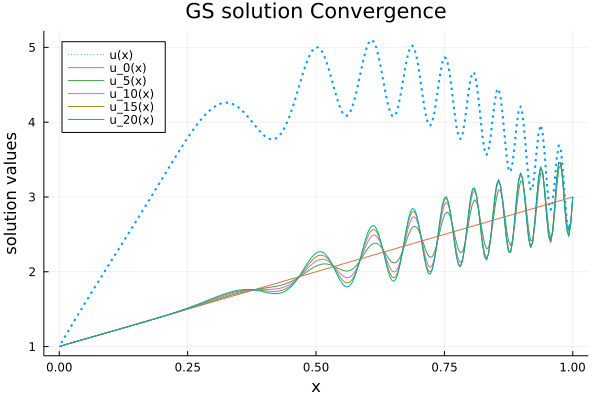
\includegraphics[width=10cm]{p2_gs_solns.png}
        \end{center}
        And the plot of the errors for each of the solution is: 
        \begin{center}
            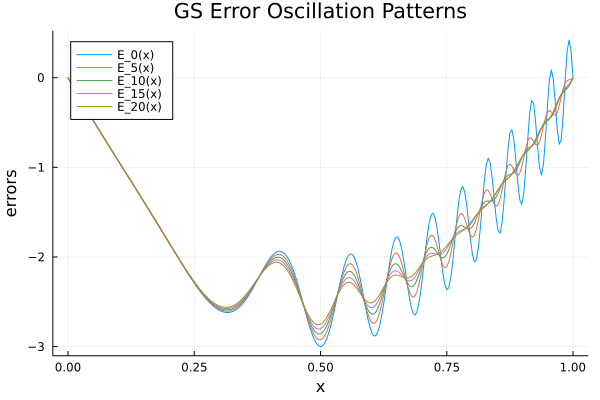
\includegraphics[width=10cm]{p2_gs_errors.png}
        \end{center}
        Please observe that the error is getting smoother and smoother as higher frequencies of oscilations are wiped away by the iterative methods. Finally, this is a list for the Inf Norm of the errors: 
        \begin{verbatim}
err: 0.1875
err: 0.1827841933736352
err: 0.1787560123586121
err: 0.1753054397389111
err: 0.17228048081525071
        \end{verbatim}
    \subsection*{CG Solutions}
        The plot of the solution found by CG during iterations: 0, 5, 10, 15, 20 is: 
        \begin{center}
            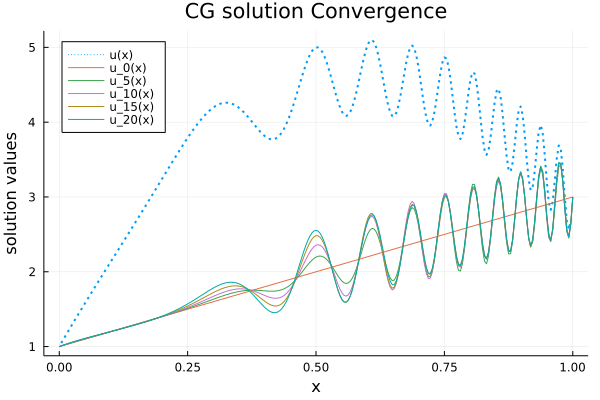
\includegraphics[width=10cm]{p2_cg_solns.png}
        \end{center}
        The plot of the error of the solution found by CG for solution at the same iteration is plotted: 
        \begin{center}
            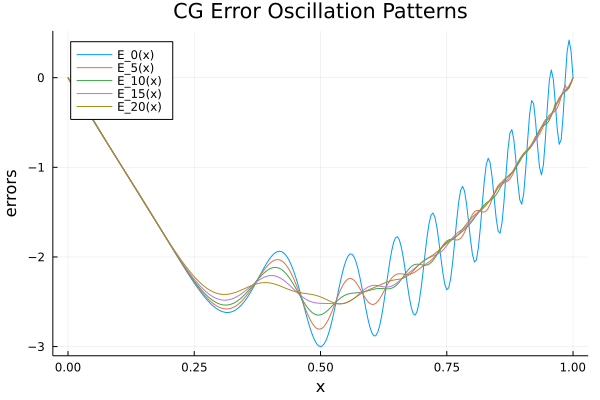
\includegraphics[width=10cm]{p2_cg_errors.png}
        \end{center}
        Observe that the same type of smoothing of the high frequencies oscilations of the solution exists for CG as well. Here is the list of errors for the solution found by cg at these key iterations: 
        \begin{verbatim}
err: 0.1875
err: 0.1753017032952856
err: 0.16554214673565795
err: 0.15765193211388995
err: 0.15774519163539247
        \end{verbatim}



\section*{Problem 3}
    
\section*{Problem 4}
    \subsection*{4(a)}
        
    \subsection*{4(b)}


\end{document}